% Created 2020-07-13 lun 10:36
% Intended LaTeX compiler: pdflatex
\documentclass[presentation,aspectratio=169]{beamer}
\usepackage[utf8]{inputenc}
\usepackage[T1]{fontenc}
\usepackage{graphicx}
\usepackage{grffile}
\usepackage{longtable}
\usepackage{wrapfig}
\usepackage{rotating}
\usepackage[normalem]{ulem}
\usepackage{amsmath}
\usepackage{textcomp}
\usepackage{amssymb}
\usepackage{capt-of}
\usepackage{hyperref}
\usepackage{khpreamble}
\usepackage{amssymb}
\DeclareMathOperator{\shift}{q}
\DeclareMathOperator{\diff}{p}
\usetheme{default}
\author{Kjartan Halvorsen}
\date{\today}
\title{Control computarizado - Asignaciónde polos (RST posicional)}
\hypersetup{
 pdfauthor={Kjartan Halvorsen},
 pdftitle={Control computarizado - Asignaciónde polos (RST posicional)},
 pdfkeywords={},
 pdfsubject={},
 pdfcreator={Emacs 26.3 (Org mode 9.3.6)}, 
 pdflang={English}}
\begin{document}

\maketitle

\section{Intro}
\label{sec:org5a20044}

\begin{frame}[label={sec:org6525fbb}]{Objetivo}
\begin{itemize}
\item Entender diseño de un controlador por asignación de polos
\end{itemize}
\end{frame}

\section{2-dof controller}
\label{sec:org6b1dd2c}

\begin{frame}[label={sec:org77445c9}]{Controlador de dos grados de libertad}
\begin{center}
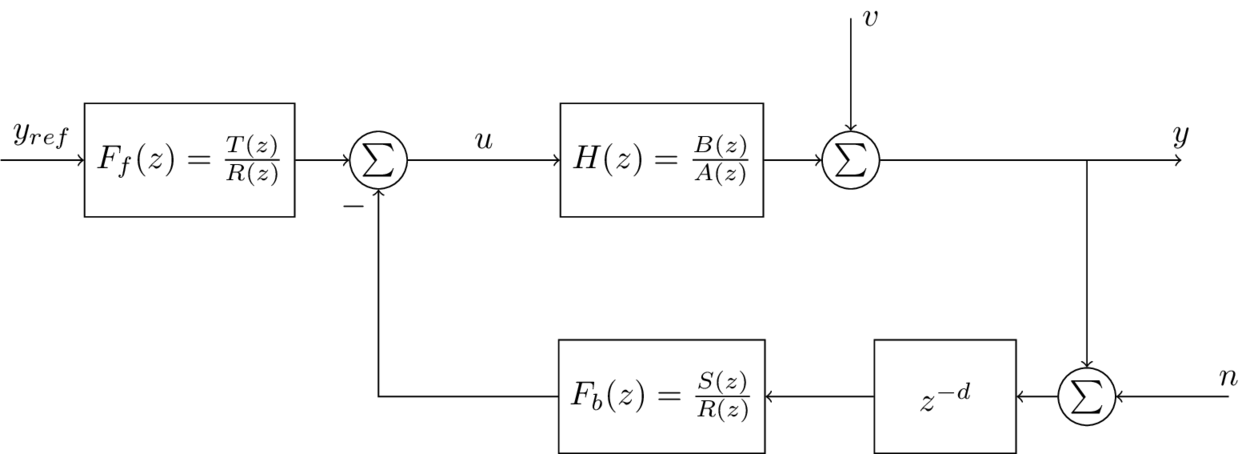
\includegraphics[width=0.8\linewidth]{../../figures/2dof-block-explicit}
\end{center}
\end{frame}

\section{RST}
\label{sec:org4389793}

\begin{frame}[label={sec:org9ec9e5d}]{Procedimiento}
Dado modelo del proceso \(H(z)=\frac{B(z)}{A(z)}\), y specificaciones de polos deseados del sistema en lazo cerrado \(A_{cl}(z) = (z-\alpha_1)(z-\alpha_2) \cdots (z-\alpha_{n_c})\)
\begin{enumerate}
\item Determina la ecuación diofántica
\[ A(z)R(z)z^{d} + B(z)S(z) = A_{cl}(z) \]
\item Determina polinomios \(R(z)\) y \(S(z)\) donde \(n_R \ge n_S\) que satisfican
\[ A(z)R(z)z^{d} + B(z)S(z) = A_{cl}(z) \]
\item Factoriza el polinomio caracteristico del lazo cerrado \(A_{cl}(z) = A_c(z)A_o(z)\), donde \(n_{A_o} \le n_R\). Eliga
\[T(z) = t_0 A_o(z),\] donde \(t_0 = \frac{A_c(1)}{B(1)}\).
\end{enumerate}

Nos da el ley de control 
\[ R(q) u(k) = T(q)u_c(k) - S(q)y(k). \]
y la respuesta en lazo cerrado a la señal de referencia
\[ A_c(q)y(k) = t_0 B(q) u_c(k). \]
\end{frame}
\begin{frame}[label={sec:org96b8351}]{Determining the order of the controller}
With Diophantine equation 
   \[ A(z)R(z)z^{d} + B(z)S(z) = A_{cl}(z) \qquad (*) \]
and feedback controller
\[F_b(z) = \frac{S(z)}{R(z)} = \frac{s_0z^n + s_1z^{n-1} + \cdots + s_n}{z^n + r_1 z^{n-1} + \cdots + r_n}\]
\alert{How should we choose the order of the controller?} Note:
\begin{itemize}
\item the controller has \(n+n+1 = 2\deg R + 1\) unknown parameters
\item the LHS of \((*)\) has degree \(\deg \big(A(z)R(z)z^d + B(z)S(z)\big) = \deg A + \deg R + d\)
\item The diophantine gives as many (nontrivial) equations as the degree of the polynomials on each side when we set the coefficients equal.

\alert{\(\Rightarrow\;\)Choose \(\deg R\) so that \(2\deg R + 1 = \deg A + \deg R + d\)}
\end{itemize}
\end{frame}


\begin{frame}[label={sec:org658f8e5}]{Determining the order of the controller - Exercise 1}
With the plant model \[H(z) = \frac{B(z)}{A(z)} = \frac{b}{z + a}\] and \(d=0\) (no delay), what is the appropriate degree of the controller 
\[F_b(z) = \frac{S(z)}{R(z)} = \frac{s_0z^n + s_1z^{n-1} + \cdots + s_n}{z^n + r_1 z^{n-1} + \cdots + r_n}\]
so that all parameters can be determined from the diophantine equation
\[ A(z)R(z) + B(z)S(z) = A_c(z)A_o(z)?\]
\begin{center}
\begin{tabular}{ll}
1. \(n = 0\) & 2. \(n = 1\)\\
3. \(n=2\) & 4. \(n=3\)\\
\end{tabular}
\end{center}
\end{frame}

\begin{frame}[label={sec:orga998746}]{Determining the order of the controller - Exercise 1}
With the plant model \[H(z) = \frac{B(z)}{A(z)} = \frac{b}{z + a}\] and \(d=0\) (no delay), what is the appropriate degree of the controller \[F_b(z) = \frac{S(z)}{R(z)} = \frac{s_0z^n + s_1z^{n-1} + \cdots + s_n}{z^n + r_1 z^{n-1} + \cdots + r_n}\]
so that all parameters can be determined from the diophantine equation
\[ A(z)R(z) + B(z)S(z) = A_c(z)A_o(z)?\]
\begin{center}
\begin{tabular}{rr}
1. \(n = 0\) & 2.\\
3. & 4.\\
\end{tabular}
\end{center}
\end{frame}

\begin{frame}[label={sec:org9492b58}]{Determining the order of the controller - Exercise 2}
With the plant model \[H(z) = \frac{B(z)}{A(z)} = \frac{b_0z + b_1}{z^2 + a_1z + a_2}\] and \(d=2\), what is the appropriate degree of the controller \[F_b(z) = \frac{S(z)}{R(z)} = \frac{s_0z^n + s_1z^{n-1} + \cdots + s_n}{z^n + r_1 z^{n-1} + \cdots + r_n}\]
so that all parameters can be determined from the diophantine equation
\[ A(z)R(z)z^2 + B(z)S(z) = A_c(z)A_o(z)?\]
\begin{center}
\begin{tabular}{ll}
1. \(n = 1\) & 2. \(n = 2\)\\
3. \(n=3\) & 4. \(n=4\)\\
\end{tabular}
\end{center}
\end{frame}

\begin{frame}[label={sec:orgd64b1c6}]{Determining the order of the controller - Exercise 2}
With the plant model \[H(z) = \frac{B(z)}{A(z)} = \frac{b_0z + b_1}{z^2 + a_1z + a_2}\] and \(d=2\), what is the appropriate degree of the controller \[F_b(z) = \frac{S(z)}{R(z)} = \frac{s_0z^n + s_1z^{n-1} + \cdots + s_n}{z^n + r_1 z^{n-1} + \cdots + r_n}\]
so that all parameters can be determined from the diophantine equation
\[ A(z)R(z)z^2 + B(z)S(z) = A_c(z)A_o(z)?\]
\begin{center}
\begin{tabular}{rr}
1. & 2.\\
3. \(n=3\) & 4.\\
\end{tabular}
\end{center}
\end{frame}

\begin{frame}[label={sec:org876a703}]{Determining the order of the controller - Exercise 3}
With the plant model \[H(z) = \frac{B(z)}{A(z)} = \frac{b_0z + b_1}{z^2 + a_1z + a_2}\] and \(d=2\)    the appropriate degree of the controller is 3 
\[F_b(z) = \frac{S(z)}{R(z)} = \frac{s_0z^3 + s_1z^2 + s_2z + s_3}{z^3 + r_1 z^2 + r_2z + r_3}.\]
What are the possible choices of the degree of the observer polynomial \(A_o(z)\) in
\[ A(z)R(z)z^2 + B(z)S(z) = A_c(z)A_o(z)?\]
\begin{center}
\begin{tabular}{ll}
1. less than 2 & 2. less than 3\\
3. higher than 2 & 4. less than or equal to 3\\
\end{tabular}
\end{center}
\end{frame}

\begin{frame}[label={sec:org7f86042}]{Determining the order of the controller - Exercise 3}
With the plant model \[H(z) = \frac{B(z)}{A(z)} = \frac{b_0z + b_1}{z^2 + a_1z + a_2}\] and \(d=2\)    the appropriate degree of the controller is 3
\[F_b(z) = \frac{S(z)}{R(z)} = \frac{s_0z^3 + s_1z^2 + s_2z + s_3}{z^3 + r_1 z^2 + r_2z + r_3}.\]
What are the possible choices of the degree of the observer polynomial \(A_o(z)\) in
\[ A(z)R(z)z^2 + B(z)S(z) = A_c(z)A_o(z)?\]
\begin{center}
\begin{tabular}{rr}
1. & 2.\\
3. & 4. less than or equal to 3\\
\end{tabular}
\end{center}
\end{frame}

\begin{frame}[label={sec:orgb7daa22}]{Where to place the closed-loop poles?}
\begin{center}
\begin{tabular}{cc}
 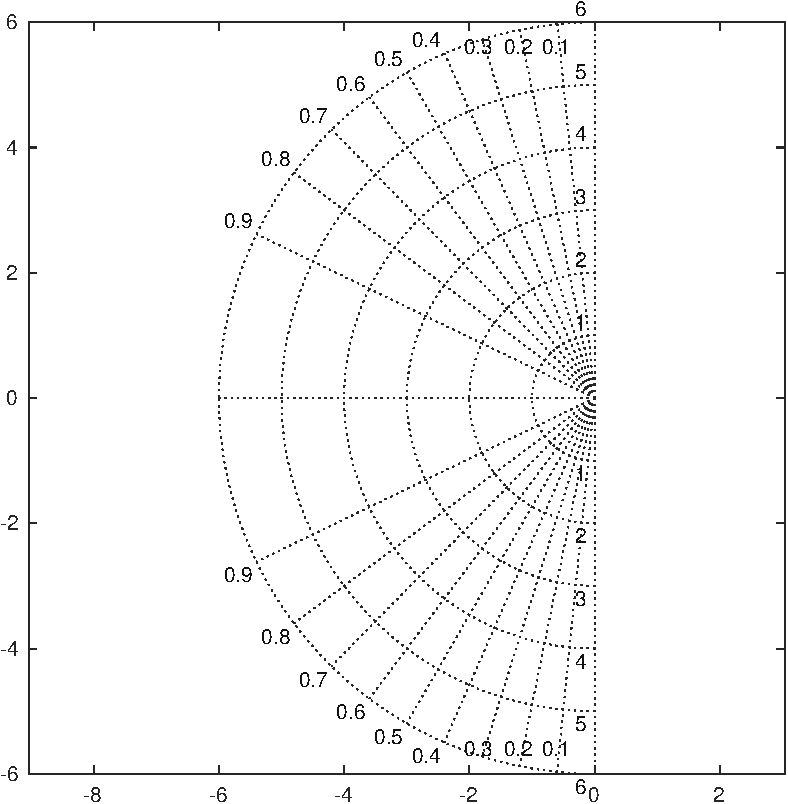
\includegraphics[width=0.41\linewidth]{../../figures/sgrid-crop}
& 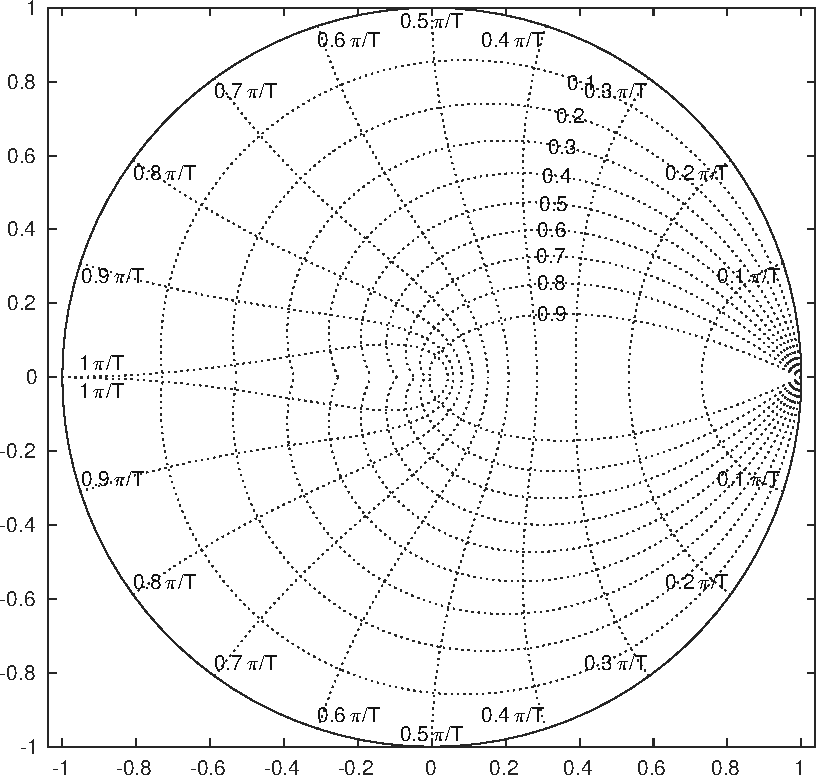
\includegraphics[width=0.43\linewidth]{../../figures/zgrid-crop}\\
s-plane & z-plane
\end{tabular}
\end{center}
\end{frame}
\end{document}